\documentclass{article}
\usepackage[utf8]{inputenc}
\usepackage[ngerman]{babel}
\usepackage[T1]{fontenc}
\usepackage{lmodern}
\usepackage{graphicx}
\usepackage[locale=DE]{siunitx}
\usepackage{float}
\usepackage[nottoc,numbib]{tocbibind}
\newcommand{\RM}[1]{\MakeUppercase{\romannumeral #1}}


\usepackage{longtable}

\usepackage{bibgerm}

\usepackage{footnpag}

\usepackage{ifthen}

\usepackage{graphicx}

\usepackage{here}

\usepackage{amsmath}

\usepackage{amsxtra}

\usepackage{amsfonts}

\usepackage{amssymb}

\usepackage{url}

%Für Testzwecke aktivieren, zeigt labels und refs im Text an.

%\usepackage{showkeys}

% Abstand zwischen zwei Absätzen nach DIN (1,5 Zeilen)

\setlength{\parskip}{1.5ex plus0.5ex minus0.5ex}

% Einrückung am Anfang eines neuen Absatzes nach DIN (keine)

\setlength{\parindent}{0pt}

% Ränder definieren

\setlength{\oddsidemargin}{0.3cm}

\setlength{\textwidth}{15.6cm}

% bessere Bildunterschriften

\usepackage[center]{caption2}

% Problemlösungen beim Umgang mit Gleitumgebungen

\usepackage{float}

% Nummeriert bis zur Strukturstufe 3 (also <section>, <subsection> und <subsubsection>)

\setcounter{secnumdepth}{3}

% Führt das Inhaltsverzeichnis bis zur Strukturstufe 3

\setcounter{tocdepth}{3}

\usepackage{exscale}





% führt mit \vv zu längenangepassten vektorpfeilen

\usepackage{esvect}

%Ergibt eine nummerierte Aufzählung bei enumerate

%\begin{compactenum}[(i)] führt zu (i), (ii), (iii), (iv), ...

%\begin{compactenum}[(I)] führt zu (I), (II), (III), (IV), ...

%\begin{compactenum}[a)] führt zu a), b), c), d), ...

\usepackage{paralist}


\newenvironment{dsm} {\begin{displaymath}} {\end{displaymath}}

\newenvironment{vars} {\begin{center}\scriptsize} {\normalsize \end{center}}

\newcommand {\en} {\varepsilon_0} % Epsilon-Null aus der Elektrodynamik

\newcommand {\lap} {\; \mathbf{\Delta}} % Laplace-Operator

\newcommand {\R} { \mathbb{R} } % Menge der reellen Zahlen

\newcommand {\e} { \ \mathbf{e} } % Eulersche Zahl

\renewcommand {\i} { \mathbf{i} } % komplexe Zahl i

\newcommand {\N} { \mathbb{N} } % Menge der nat. Zahlen

\newcommand {\C} { \mathbb{C} } % Menge der kompl. Zahlen

\newcommand {\Z} { \mathbb{Z} } % Menge der kompl. Zahlen

\newcommand {\limi}[1]{\lim_{#1 \rightarrow \infty}} % Limes unendlich

\newcommand {\sumi}[1]{\sum_{#1=0}^\infty}

\newcommand {\rot} {\; \mathrm{rot} \,} % Rotation

\newcommand {\grad} {\; \mathrm{grad} \,} % Gradient

\newcommand {\dive} {\; \mathrm{div} \,} % Divergenz

\newcommand {\dx} {\; \mathrm{d} } % Differential d

\newcommand {\cotanh} {\; \mathrm{cotanh} \,} %Cotangenshyperbolicus

\newcommand {\asinh} {\; \mathrm{areasinh} \,} %Area-Sinus-Hyp.

\newcommand {\acosh} {\; \mathrm{areacosh} \,} %Area-Cosinus-H.

\newcommand {\atanh} {\; \mathrm{areatanh} \,} %Area Tangens-H.

\newcommand {\acoth} {\; \mathrm{areacoth} \,} % Area-cotangens

\newcommand {\Sp} {\; \mathrm{Sp} \,}

\newcommand {\mbe} {\stackrel{\text{!}}{=}} %Must Be Equal

\newcommand{\qed} { \hfll $\square$\\}

\renewcommand{\i} {\imath}

\newcommand{\ham}{\mathcal{H}}

\newcommand{\lag}{\mathcal{L}}

\def\captionsngerman{\def\figurename{\textbf{Abb.}}}

\renewcommand{\dagger}{**}

\renewcommand{\contentsname}{Inhaltsverzeichnis}

\renewcommand{\figurename}{Abbildung}

\renewcommand{\tablename}{Tabelle}

%\scriptsize \Large

\begin{document}
	\scriptsize \normalsize
	\title{ Tomographie mittels $\gamma$-Strahlung  \\ Versuch 14}
	

	
	\author{Polina Stecher\\ {polina.stecher@tu-dortmund.de}  \and   Sonya Djuffouo Tchinda\\ {sonya.djuffouo@tu-dortmund.de}} %{polina.stecher@tu-dortmund.de  sonya.djuffouo@tu-dortmund.de} 
	\date{Durchgeführt am  19. Juni  2018}
		\maketitle
	\newpage
	\tableofcontents
	\thispagestyle{empty}
	\newpage
	\newpage
	
\section{Einleitung }

Im folgenden Versuch wird mit Hilfe der Tomographie ein Würfel, welches aus 27 Elementarwürfeln zusammengesetzt ist, auf seine Materialien untersucht. Dieser wird von $\gamma$- Strahlung in verschiedenen Einstrahlwinkel durchstrahlt. Anhand der Absorption der Strahlung lassen sich Rückschlüsse auf die enthalteten Stoffe ziehen. 

\section{Theorie} 

\subsection{Tomographie allgemein}

Die Tomographie ist allgemein ein bildgebendes Verfahren und dient zur Untersuchung räumlicher Strukturen mit Hilfe von Querschnittbilder. Dabei wird das zu untersuchende Objekt mit $\gamma$- Strahlung bestrahlt und die Intensität der Strahlung vor und nach der Transmission durch ein Objekt gemessen. Die Strahlung wird je nach Material unterschiedlich stark absorbiert aufgrund der unterschiedlichen Absorptionskoeffizienten $\mu_i$. Die Zählrate N hinter der Probe lässt sich mit Hilfe der Formel:
\begin{align}
N=N_0 e^{-\sum \mu_i d_i}
\end{align}
$N_0$ ist die Anfangszählrate, $d_i$ ist die Wegstrecke und $\mu_i$ sind die Absorptionskoeffizienten. Um ein dreidimensionales Bild zu erzeugen, werden verschiedene Projektionen aus unterschiedlichen Richtungen benötigt. Um aus dem Gleichungssystem die Absorptionskoeffizienten zu bestimmen, wird ein überbestimmtes Gleichungssystem benötigt. Es ergibt sich eine Matrixgleichung
\begin{align}
A\vec{\mu}^T= \vec{I}
\end{align}

Es gilt $A_{ji}=d_{ji}$ und $I_i=ln \left(\dfrac{N_0}{Ni} \right)$. Die Gleichung (2) wird nach $\mu$ umgestellt und es ergibt sich die Lösung: 
\begin{align}
\vec{\mu}= (A^T A)^{-1}  A^T I
\end{align}	
\subsection{Spektrum der Quelle}
Als Quelle wird das Element $^{137}$Cs benutzt. Cäsium ist ein Alkalimetall, das durch einen $\beta^-$ -Zerfall in matastabildes Barium-137 zerfällt. Das metastabile Barium-137 zerfällt durch Aussendung eines $\gamma$-Quants mit einer Energie von 662 keV in stabiles Barium-137. Das Spektrum ist in der Abbildung (1) dargestellt. 

 \begin{figure}[H]
	\centering
	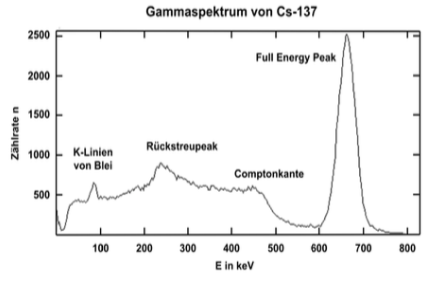
\includegraphics[height=5cm, width=8cm]{hallo.png}
	\caption{ Spektrum der verwendeteten Quelle $^{[1]}$}   
	\label{fig: abb. 1}
\end{figure}
Das Hauptmaximum des Spektrums liegt etwa bei 662keV. Dieses ist der sogenannte Full-Energy-Peak, welches durch die vollständige Energieabgabe des Photons an das Elektron im Detektor entsteht. Beim Comptoneffekt wird die Energie nur teilweise an das Elektron übertragen. Das Comptonkontinuum welches sich im linken Bereicht der Abbildung (1) erstreckt, entsteht durch Streuung der Photonon.

\subsection{Wechselwirkung von $\gamma$-Strahlung mit Materie}

Die Proben werden mit $^\gamma$-Strahlung durchstrahlt. Die Absorption/Abschwächung der Strahlung in Materie entsteht durch verschiedene Wechselwirkungen. Beim Comptoneffekt trifft das Photon auf ein freies Elektron und vollführt einen inalstischen Stoß. Dabei gibt das Photon ein Teil seiner Energie ab und ändert dabei seine Geschwindigkeitsrichtung. Durch die Energieübertragung kommt es zu einer Wellenlängenänderung des Photons nach dem Stoß. Beim Photoeffekt trifft das Phton auf ein festes Elektron und gibt dabei seine gesamte Energie an das Elektron ab. Wenn die Energie des Photons genau der Bindungsenergie des Elektrons enspricht, wird das Elektron aus dem Atom gelöst. Bei der Paabildung wird durch die Aufnahme eines Impulses der auftreffenden Photonenstrahlung durch den Atomkern Strahlung in Materie verwandelt. Dabei bildet sich ein Elektron-Positron-Paar. Dieser Effekt spielt jedoch bei den in diesem Versuch verwendeteten Energien keine Rolle. 

\section{Aufbau und Durchführung}

Der Versuchsaufbau, bestehend aus der Cäsium -Probe als $\gamma$-Quelle, den zu untersuchenden Würfeln und dem NaJ-Detektor sind in der Abbildung 2 zu sehen. 

\begin{figure}[H]
	\centering
	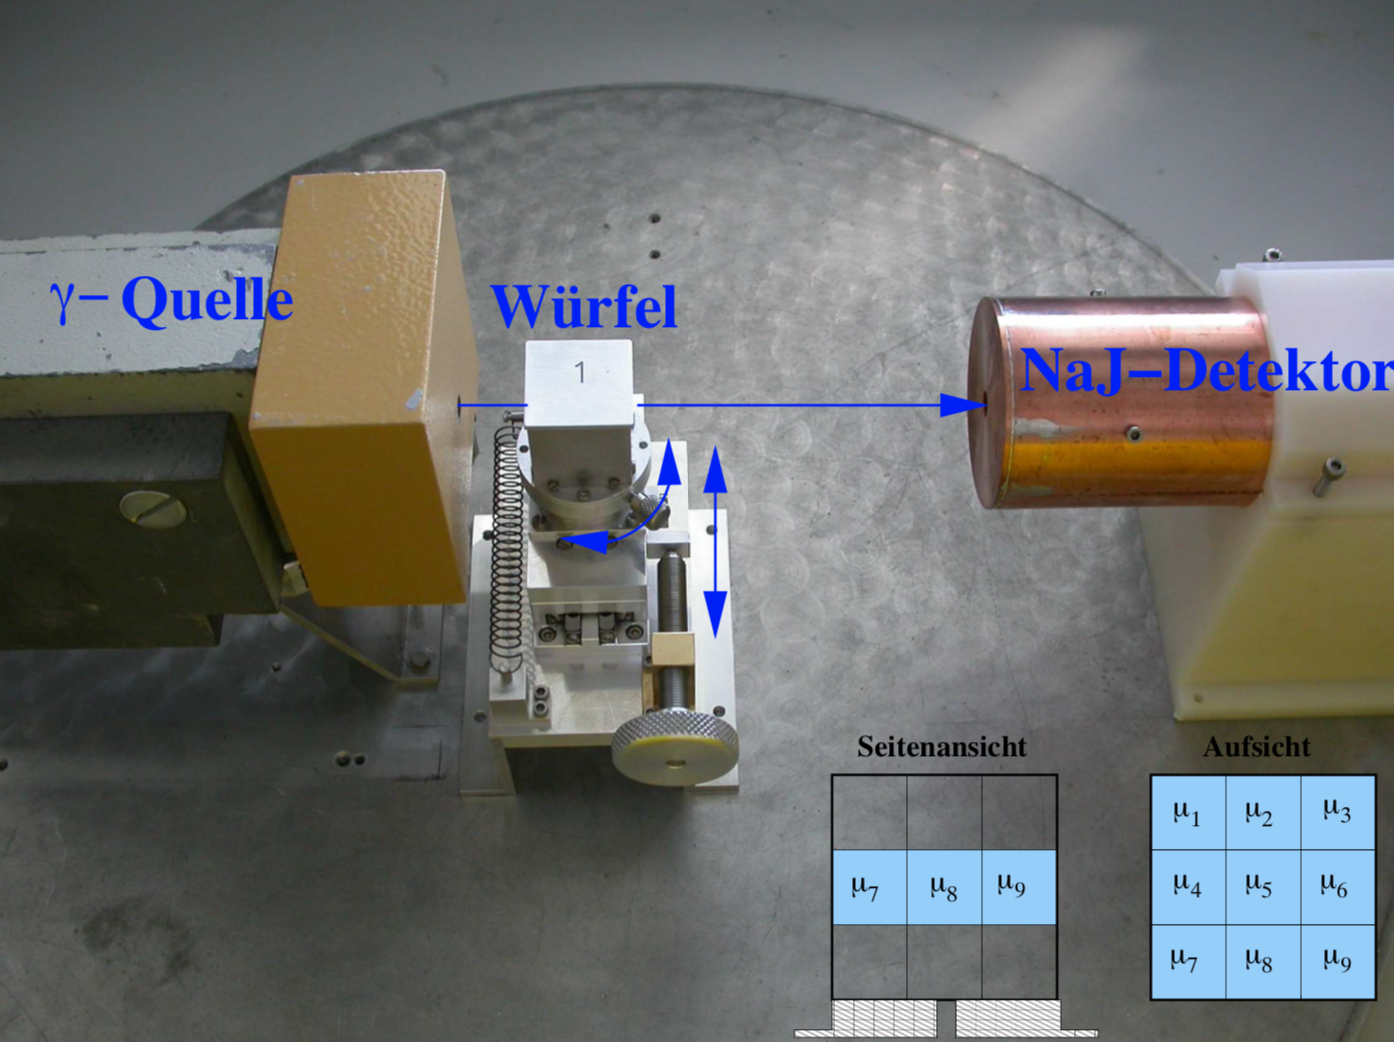
\includegraphics[height=5cm, width=8cm]{aufbau.png}
	\caption{ Versuchsaufbau $^{[2]}$}   
	\label{fig: abb. 1}
\end{figure}



Zur Detektion wird ein Szintillationsdetektor mit einem Vielkanalanalysator verwendet. Im Kopf befindet sich ein von äußerem Licht geschützter NaJ-Kristall. Die einfallende Strahlung regt die Atome des Kristalls an, sodass diese Photone ausstrahlen. Die ausgesendeten Photonen gelangen in den Photomultiplier. Dort befindet sich eine Photokathode, aus der durch den Photoeffekt Elektronen ausgelöst werden, die daraufhin von einer Spannung beschleunigt werden und ein Vielfaches an Elektronen auslösen. An der Anode kann dann ein gut messbarer Stromimpuls gemessen werden, dessen Amplitude von der Energie der einfallenden Strahlung abhängig ist. Die Impulse treten in den Multichannelanalyzer, wo sie nach ihrer Größe und ihrer Häufigkeit sortiert werden und anschließend ein Histogramm der Intensitätsverteilung  erstellt wird. 

Der Strahl trifft auf den aus 27 Elementarwürfeln bestehenden Würfel, der in einer Halterung befestigt und in der richtigen Projektionsrichtung justiert wird. Anschließend werden die nicht absorbierten Strahlen über einen Zeitintervall von ca. 300 Sekunden vom Detektor aufgenommen. Zunächst wird eine Messung des Aluminiumgehäuses durchgeführt, um die Eingangsintensität $N_0$ zu bestimmen. Dazu wird eine gerade und eine schräge Projektion ausgewählt.  Daraufhin werden zwei weitere Würfel (2 und 3), die jeweils aus einem Material bestehen,  aus verschiedenen Projektionen untersucht. Zuletzt wird der Würfel 4 untersucht. Dieser besteht aus mehreren zusammengesetzten Materialien. Die bei der Messung verwendeten Projektionen sind in der Abbildung (3) schematisch dargestellt. 


\end{document}